% ==============================================================================
%                                    DVG303
%                  Objektorienterad design och programmering
%                                Laboration #2
%
% Author:   Jonas Sjöberg
%           Högskolan i Gävle
%           tel12jsg@student.hig.se
%           https://github.com/jonasjberg
%
% License:  Creative Commons Attribution-NonCommercial-ShareAlike 4.0
%           International.  See LICENSE.md for full licensing information.
% ==============================================================================

\section{Uppgift 1}\label{sec:uppg1}

\subsection{}\label{sec:uppg1a}
\subsubsection*{Frågeställning}
I laboration 1 definierade ni redan emph{ett} interface. Kontrollera om
interfacet passar in i mönstret som beskrevs ovan och gör ändringar ifall
interfacet måste anpassas.

\subsubsection*{Lösning}
Ett nytt paket \texttt{component} (\texttt{se.hig.oodp.lab.model.component})
innehåller de tre interface som ska användas för att manipulera alla typer av
figurer; \texttt{Movable}, \texttt{Rotatable} och \texttt{Scalable}.
Dessa tre interface skapades i den förra laborationen och har inte ändrats.


\subsection{}\label{sec:uppg1b}
\subsubsection*{Frågeställning}
Modellera alla interfacen som behövs utöver interfacet från
Uppgift~\ref{uppg1a} (beskrivning och UML-diagram; uppdatera klassdiagrammet).

\subsubsection*{Lösning}
Uppdaterade UML-diagram återfinns i Figur~\ref{fig:uppg1b1} samt
Figur~\ref{fig:uppg1b2}.

\begin{sidewaysfigure}[ht]
\centering
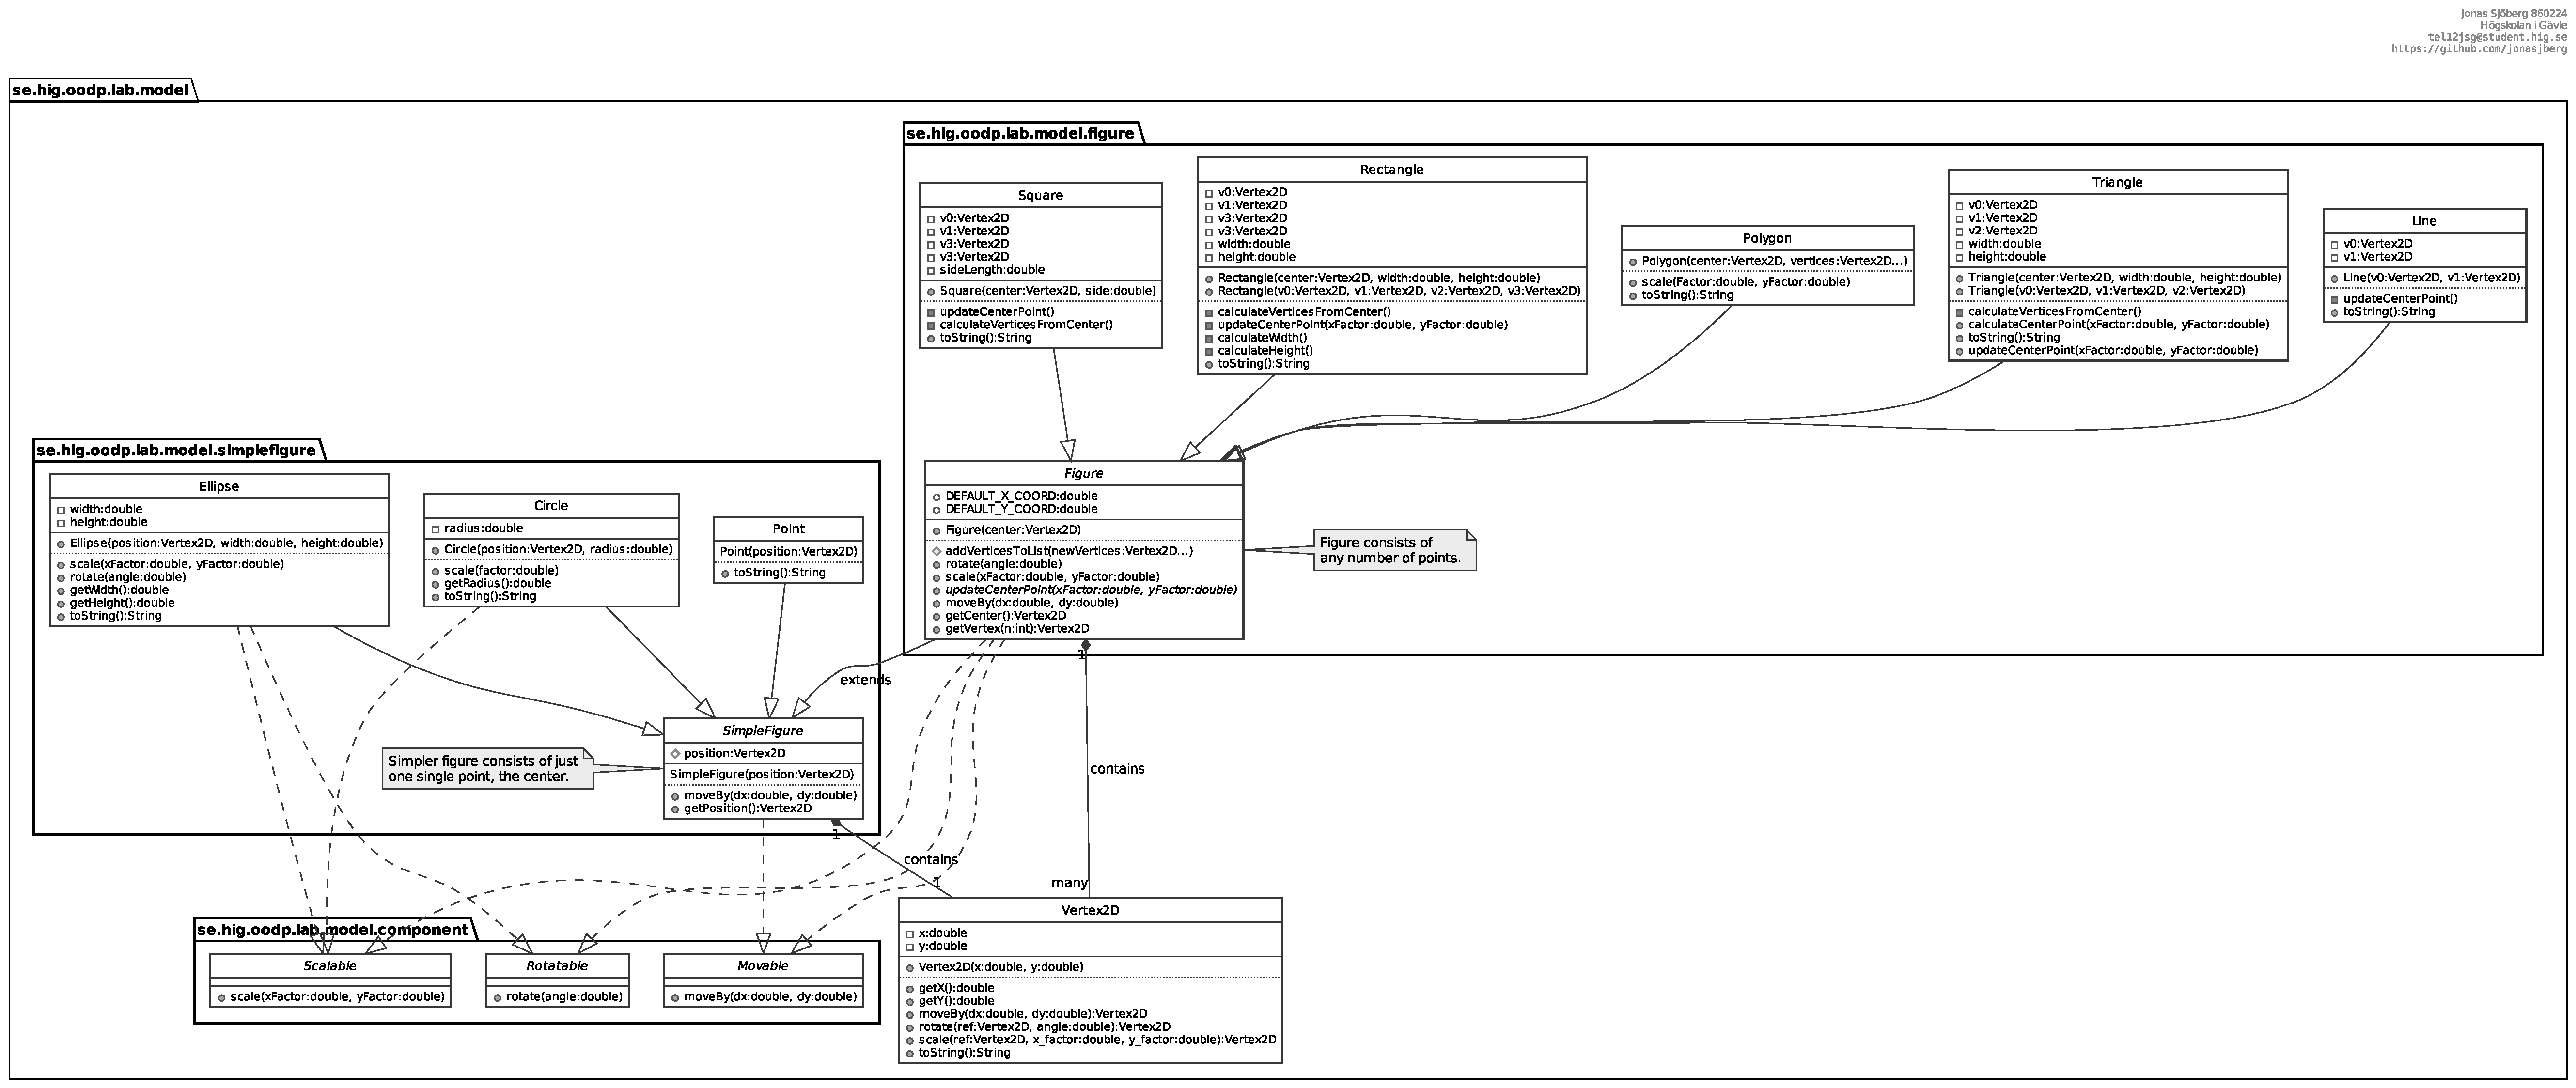
\includegraphics[width=\linewidth]{diagram/lab2-uppgift1-001.eps}
\caption{Uppdaterat UML-diagram, sida 1 av 2.
%(\texttt{diagram/lab2-uppgift1-001.eps})
}
\label{fig:uppg1b1}
\end{sidewaysfigure}

\begin{sidewaysfigure}[ht]
\centering
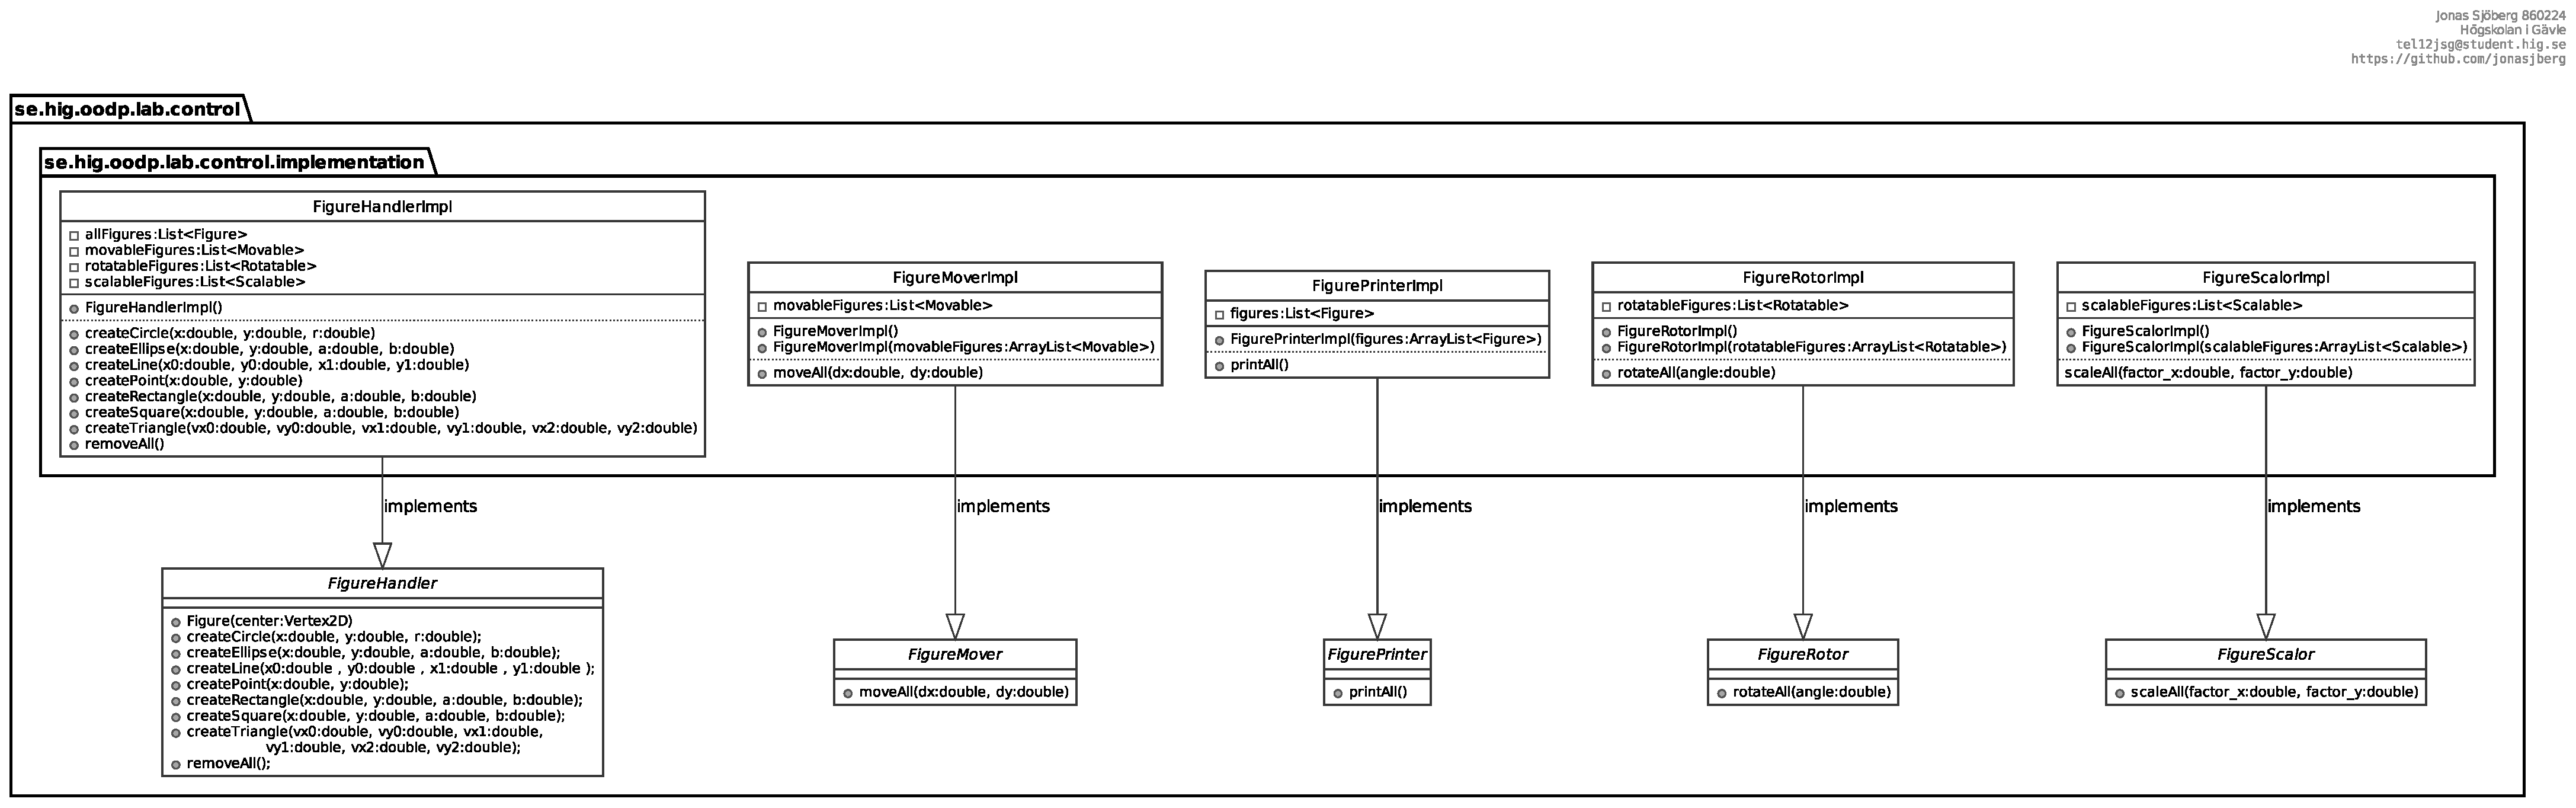
\includegraphics[width=\linewidth]{diagram/lab2-uppgift1-002.eps}
\caption{Uppdaterat UML-diagram, sida 2 av 2.
%(\texttt{diagram/lab2-uppgift1-002.eps})
}
\label{fig:uppg1b2}
\end{sidewaysfigure}


\subsection{}\label{sec:uppg1c}
\subsubsection*{Frågeställning}
Skriv interfacen från Uppgift~\ref{sec:uppg1b} i Java.

\subsubsection*{Lösning}
Se bifogad källkod.

%\subsubsubsection{Movable.java}
%\javacode{src/se/hig/oodp/lab/model/component/Movable.java}
%\caption{Interfacet Movable}
%\label{src:movable}

%\subsubsubsection{Rotatable.java}
%\javacode{src/se/hig/oodp/lab/model/component/Rotatable.java}
%\caption{Interfacet Rotatable}
%\label{src:rotatable}

%\subsubsubsection{Scalable.java}
%\javacode{src/se/hig/oodp/lab/model/component/Scalable.java}
%\caption{Interfacet Scalable}
%\label{src:scalable}



%% Screenshots med Bash, terminalfönsterstorlek 90x40
%\subsection{Skärmdump}
%Se Figur~\ref{fig:uppg01-screenshot} för skärmdump på körning av koden i
%Sektion~\ref{src:uppg01} och Sektion~\ref{src:userinputfilter}.
%
%\begin{figure}[htbp]
%\centering
%\includegraphics[width=\linewidth]{img/01.png}
%\caption{Körning av koden till Uppgift~\ref{sec:uppg01}}
%\label{fig:uppg01-screenshot}
%\end{figure}

